\documentclass{ximera}

\usepackage{microtype}
\usepackage{tikz}
\usepackage{tkz-euclide}
\usetkzobj{all}
\tikzstyle geometryDiagrams=[ultra thick,color=blue!50!black]

\renewcommand{\epsilon}{\varepsilon}



\title{Central projection}
\begin{document}
\begin{abstract}
Here we start to develop unified models for our geometries.
\end{abstract}
\maketitle

\section{Central projection coordinates}

Let's project $K$-geometry,
\[
1=K\left(x^{2}+y^{2}\right)+z^{2} 
\]
onto the plane $z=1$ using the origin $O=(0,0,0)$ as the center of
projection:
\[
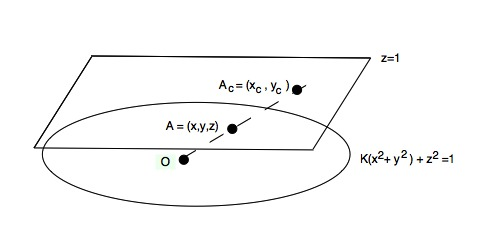
\includegraphics[width=3in]{MXAJBZ0K.jpg}
\qquad
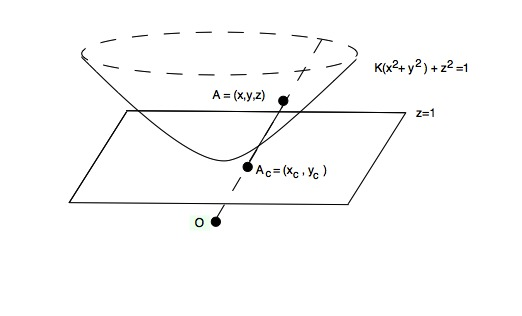
\includegraphics[width=3in]{MXAJBZ0L.jpg}
\]
Let's look at this from a different vantage point, say with our eye parallel to the plane $z=1$.
\[
\text{IMAGE: side view with $\lambda$ labeled}
\]
Note, we are only projecting the top of the surface
\[
1=K\left(x^{2}+y^{2}\right)+z^{2} 
\]
onto the plane $z=1$. So when $K>0$, this is the ``Northern hemisphere'' of
the sphere, when $K<0$, this is the upper hyperboloid, and when $K=0$,
this is the plane $z=1$.

\begin{problem}
  What range of values could $\lambda$ take when $K>0$?
  \begin{freeResponse}
    In this case, $\lambda\in (0,1)$.
  \end{freeResponse}
\end{problem}

\begin{problem}
  What range of values could $\lambda$ take when $K<0$?
  \begin{freeResponse}
    In this case, $\lambda\in(1,\infty)$.
  \end{freeResponse}
\end{problem}

\begin{problem}
  What range of values could $\lambda$ take when $K=0$?
  \begin{freeResponse}
    In this case
    \[
    1=K\left(x^{2}+y^{2}\right)+z^{2} 
    \]
    is the plane $z = 1$, hence $\lambda=1$.
  \end{freeResponse}
\end{problem}

\begin{problem}
  Letting $(x_c,y_c,1)$ be the image of the $K$-geometry points
  $(x,y,z)$ in the plane $z=1$, use facts about similar triangles to
  explain why
  \[
  \lambda\cdot(x_{c},y_{c},1)=(x,y,z).
  \]
\end{problem}


\begin{problem}
  For the projection of the set $1=K\left(x^{2}+y^{2}\right)+z^{2}$
  onto the $z=1$ plane with center of projection $O$, write
  $(x_{c},y_{c})$ as a function of $(x,y,z)$.
  \begin{freeResponse}
    We know that
    \[
    \lambda\cdot(x_{c},y_{c},1)=(x,y,z),
    \]
    hence $\lambda=z$, and we may now write
    \begin{align*}
      x_{c} &=x/z,\\
      y_{c} &=y/z.
    \end{align*}
  \end{freeResponse}
\end{problem}

\begin{problem}
  For the projection of the set $1=K\left(x^{2}+y^{2}\right)+z^{2} $
  onto the $z=1$ plane with center of projection $O$, write $(x,y,z)$
  as a function of $(x_{c},y_{c})$.
  \begin{freeResponse}
    This is slightly more complex than the previous problem; however,
    we will begin the same way. We know that
    \[
    \lambda\cdot(x_{c},y_{c},1)=(x,y,z),
    \]
    hence $\lambda=z$, and we may now write
    \begin{align*}
      x &= x_c\cdot z,\\
      y &= y_c\cdot z,\\
      z &= z.
    \end{align*}
    Now our task is to write $z$ in terms of $x_c$ and $y_c$. Using our assignments above, write
    \begin{align*}
      1 &= K\left(x^2 + y^2\right) + z^2\\
      1 &= K\left((x_c\cdot z)^2 + (y_c\cdot z)^2\right) + z^2\\
      1 &= \left(K\left(x_c^2 + y_c^2\right)+1\right)z^2,
    \end{align*}
    and so
    \[
    z = \frac{1}{\sqrt{K\left(x_c^2 + y_c^2\right)+1}}.
    \]
    Hence
    \begin{align*}
      x &= \frac{x_c}{\sqrt{K\left(x_c^2 + y_c^2\right)+1}},\\
      y &= \frac{y_c}{\sqrt{K\left(x_c^2 + y_c^2\right)+1}},\\
      z &= \frac{1}{\sqrt{K\left(x_c^2 + y_c^2\right)+1}}.\\
    \end{align*}
  \end{freeResponse}
\end{problem}






\section{Central projection dot product}

Like we have done before, now we want to be able to find a dot product
that will allow us to compute lengths in central projection
coordinates that will agree with the $K$-dot product, and hence the
euclidean dot product.


\begin{problem}
Suppose we have a curve $X$ in $K$-warped space that is a function of
a curve $X_c$ in the plane $z=1$ space. So
\[
X_c(t) = \left( x_c(t),y_c(t)\right)
\]
and
\[
X(t) = 
\begin{cases}
  x(x_c(t),y_c(t)),\\
  y(x_c(t),y_c(t)),\\
  z(x_c(t),y_c(t)).
\end{cases}
\]
Use the chain rule to compute
\[
\dd[x]{t}, \qquad \dd[y]{t}, \qquad \dd[z]{t},
\]
in terms of $\dd[x_c]{t}$, $\dd[y_c]{t}$, $\pp[x]{x_c}$,
$\pp[y]{x_c}$, $\pp[z]{x_c}$, $\pp[x]{y_c}$, $\pp[y]{y_c}$,
and $\pp[z]{y_c}$.
  \begin{hint}
  Simply write down the answer from a previous problem with some minor
  changes.
  \end{hint}
  \begin{freeResponse}
  Write
  \begin{align*}
    \dd[x]{t} &= \left(\pp[x]{x_c},\pp[x]{y_c}\right)\bullet\left(\dd[x_c]{t},\dd[y_c]{t}\right) = \pp[x]{x_c}\cdot\dd[x_c]{t}+\pp[x]{y_c}\cdot\dd[y_c]{t}, \\
    \dd[y]{t} &= \left(\pp[y]{x_c},\pp[y]{y_c}\right)\bullet\left(\dd[x_c]{t},\dd[y_c]{t}\right) = \pp[y]{x_c}\cdot\dd[x_c]{t}+\pp[y]{y_c}\cdot\dd[y_c]{t}, \\
    \dd[z]{t} &= \left(\pp[z]{x_c},\pp[z]{y_c}\right)\bullet\left(\dd[x_c]{t},\dd[y_c]{t}\right) = \pp[z]{x_c}\cdot\dd[x_c]{t}+\pp[z]{y_c}\cdot\dd[y_c]{t}.  
  \end{align*}
\end{freeResponse}
\end{problem}




\begin{problem}
  With the same setting as in the previous problem, rewrite the result
  of your computation in matrix notation to find $D_c$
  such that
\[
\begin{bmatrix}
\dd[x]{t} & \dd[y]{t} & \dd[z]{t}
\end{bmatrix}
=
\begin{bmatrix}
\frac{dx_c}{dt} & \frac{dy_c}{dt}
\end{bmatrix}\cdot D_c.
\]
\begin{hint}
  Simply write down the answer from a previous problem with some minor
  changes.
\end{hint}
\begin{freeResponse}
  \[
  D_c =
  \begin{bmatrix}
    \pp[x]{x_c} & \pp[y]{x_c} & \pp[z]{x_c} \\
    \pp[x]{y_c}   & \pp[y]{y_c}   & \pp[z]{y_c}
  \end{bmatrix}.
  \]
\end{freeResponse}
\end{problem}




\begin{problem}
  Now find $P_c$ in terms of $K$, $\pp[x]{x_c}$, $\pp[y]{x_c}$,
  $\pp[z]{x_c}$, $\pp[x]{y_c}$, $\pp[y]{y_c}$, and $\pp[z]{y_c}$ such
  that
  \[
  \left(\dd[x]{t}, \dd[y]{t}, \dd[z]{t}\right)\bullet_K
  \left(\dd[x]{t}, \dd[y]{t}, \dd[z]{t}\right)
  =
  \begin{bmatrix}
    \dd[x_c]{t} &  \dd[y_c]{t}
  \end{bmatrix}
  \cdot P_c
  \cdot
  \begin{bmatrix}
    \dd[x_c]{t} \\  \dd[y_c]{t}
  \end{bmatrix}.
  \]
  \begin{hint}
  Simply write down the answer from a previous problem with some minor
  changes.
  \end{hint}
  \begin{freeResponse}
    Working from the $K$-dot product, we need that
    \begin{align*}
    \left(\dd[x]{t}, \dd[y]{t}, \dd[z]{t}\right)\bullet_K
    \left(\dd[x]{t}, \dd[y]{t}, \dd[z]{t}\right)
    &=
    \begin{bmatrix}
      \dd[x]{t} & \dd[y]{t} & \dd[z]{t}
    \end{bmatrix}
    \begin{bmatrix}
      1 & 0 & 0\\
      0 & 1 & 0\\
      0 & 0 & K^{-1}
    \end{bmatrix}
    \begin{bmatrix}
      \dd[x]{t} \\ \dd[y]{t} \\ \dd[z]{t}
    \end{bmatrix}\\
    &=
    \begin{bmatrix}
      \frac{dx_c}{dt} & \frac{dy_c}{dt}
    \end{bmatrix}\cdot D_{c}\cdot
    \begin{bmatrix}
      1 & 0 & 0\\
      0 & 1 & 0\\
    0 & 0 & K^{-1}
    \end{bmatrix}
    \cdot
    \left(
    \begin{bmatrix}
      \frac{dx_c}{dt} & \frac{dy_c}{dt}
    \end{bmatrix}\cdot D_{c}
    \right)^\transpose\\
    &=
    \begin{bmatrix}
      \frac{dx_c}{dt} & \frac{dy_c}{dt}
    \end{bmatrix}\cdot D_{c}\cdot
    \begin{bmatrix}
      1 & 0 & 0\\
      0 & 1 & 0\\
    0 & 0 & K^{-1}
    \end{bmatrix}
    \cdot
    D_{c}^\transpose
    \cdot \begin{bmatrix}
      \frac{dx_c}{dt} \\ \frac{dy_c}{dt}
    \end{bmatrix}.
  \end{align*}
    Hence
    \begin{align*}
      P_c &=
      \begin{bmatrix}
        \pp[x]{x_c} & \pp[y]{x_c} & \pp[z]{x_c} \\
        \pp[x]{y_c} & \pp[y]{y_c} & \pp[z]{y_c}
      \end{bmatrix}
      \begin{bmatrix}
        1 & 0 & 0\\
        0 & 1 & 0\\
        0 & 0 & K^{-1}
      \end{bmatrix}
      \begin{bmatrix}
        \pp[x]{x_c} & \pp[x]{y_c}\\ 
        \pp[y]{x_c} & \pp[y]{y_c}\\
        \pp[z]{x_c} & \pp[z]{y_c}
      \end{bmatrix}\\
      &=
      \begin{bmatrix}
        \left(\pp[x]{x_c}\right)^2 + \left(\pp[y]{x_c}\right)^2 + \left(\pp[z]{x_c}\right)^2K^{-1} & \pp[x]{x_c}\pp[x]{y_c} + \pp[y]{x_c}\pp[y]{y_c} + \pp[z]{x_c}\pp[z]{y_c} K^{-1}\\
        \pp[x]{x_c}\pp[x]{y_c} + \pp[y]{x_c}\pp[y]{y_c} + \pp[z]{x_c}\pp[z]{y_c} K^{-1}       & \left(\pp[x]{y_c}\right)^2 + \left(\pp[y]{y_c}\right)^2 + \left(\pp[z]{y_c}\right)^2K^{-1}
      \end{bmatrix}.
    \end{align*}
  \end{freeResponse}
\end{problem}


\begin{problem}
  Set
  \begin{align*}
    x(x_c,y_c) &=x/\lambda,\\
    y(x_c,y_c) &=y/\lambda,\\
    z(x_c,y_c) &=\lambda,
  \end{align*}
  and show that $P_c$ from the problem above is
  \[
  P_c =
  \begin{bmatrix}
    \left(Ky_c^2+1\right)\lambda^4 & -Kx_{c}y_{c}\lambda^4\\
    -Kx_{c}y_{c}\lambda^4 & \left(Kx_c^2+1\right)\lambda^4
  \end{bmatrix}.
\]
\begin{hint}
  To compute the partial derivatives, work in the following way:
  \begin{enumerate}
  \item Recall $x = \lambda\cdot x_c$.
  \item Note that $\pp[x]{x_c} = \lambda + x_c \cdot \pp[\lambda]{x_c}$.
    \item Express the partial derivative in terms of $\lambda$, $K$, $x_c$,
      and $y_c$.
  \end{enumerate}
\end{hint}
\begin{hint}
  When simplifying, combine the terms with the highest degree of $\lambda$
  and note that
  \[
  \lambda^{-2} = K\left(x_c^2 + y_c^2\right) + 1.
  \]
\end{hint}
\begin{freeResponse}
  Write
  \begin{align*}
    \pp[x]{x_c} &= \lambda  + x_c \cdot \pp[\lambda]{x_c}\\
    &= \lambda + x_c \cdot \pp{x_c} \left(K\left(x_c^2 + y_c^2\right)+1\right)^{-1/2}\\
    &= \lambda + x_c \cdot (-1/2)\left(K\left(x_c^2 + y_c^2\right)+1\right)^{-3/2}(2Kx_c)\\
    &= \lambda -Kx_c^2 \lambda^3.
  \end{align*}
  Similarly,
    \begin{align*}
    \pp[y]{x_c} &= y_c \cdot \pp[\lambda]{x_c}\\
    &= y_c \cdot \pp{x_c} \left(K\left(x_c^2 + y_c^2\right)+1\right)^{-1/2}\\
    &= y_c \cdot (-1/2)\left(K\left(x_c^2 + y_c^2\right)+1\right)^{-3/2}(2Kx_c)\\
    &= -Kx_cy_c \lambda^3.
    \end{align*}
   Finally, 
    \begin{align*}
    \pp[z]{x_c} &= \pp[\lambda]{x_c}\\
    &= \pp{x_c}\left(K\left(x_c^2 + y_c^2\right)+1\right)^{-1/2}\\
    &= (-1/2)\left(K\left(x_c^2 + y_c^2\right)+1\right)^{-3/2}(2Kx_c)\\
    &= -Kx_c \lambda^3.
    \end{align*}
    Now with entirely similar computations, we see
    \begin{align*}
      \pp[x]{y_c} &= -Kx_cy_c \lambda^3,\\
      \pp[y]{y_c} &= \lambda - Ky_c^2 \lambda^3,\\
      \pp[z]{y_c} &= -Ky_c \lambda^3.
    \end{align*}


    
    Now we see $\left(\pp[x]{x_c}\right)^2 + \left(\pp[y]{x_c}\right)^2 + \left(\pp[z]{x_c}\right)^2K^{-1}$
    \begin{align*}
      &= \left(\lambda -Kx_c^2 \lambda^3\right)^2 + \left(-Kx_cy_c \lambda^3\right)^2 + \left(-Kx_c \lambda^3\right)^2K^{-1}\\
      &= \lambda^2 - 2Kx_c^2\lambda^4 + K^2x_c^4 \lambda^6+ K^2x_c^2y_c^2\lambda^6 + Kx_c^2\lambda^6\\
      &= \lambda^2 - 2Kx_c^2\lambda^4 + Kx_c^2\lambda^6\left(Kx_c^2 + Ky_c^2 + 1\right)\\
      &= \lambda^2 - 2Kx_c^2\lambda^4 + Kx_c^2\lambda^6\left(K\left(x_c^2 + y_c^2\right) + 1\right)\\
      &= \lambda^2 - 2Kx_c^2\lambda^4 + Kx_c^2\lambda^6 \lambda^{-2}\\
      &= \lambda^2 - 2Kx_c^2\lambda^4 + Kx_c^2\lambda^4\\
      &= \lambda^2 - Kx_c^2\lambda^4\\
      &= \frac{1}{K\left(x_c^2+y_c^2\right)+1} - \frac{Kx_c^2}{\left(K\left(x_c^2+y_c^2\right)+1\right)^2}\\
      &= \frac{K\left(x_c^2 + y_c^2\right) +1 - Kx_c^2}{\left(K\left(x_c^2+y_c^2\right)+1\right)^2}\\
      &= \frac{Ky_c^2+1}{\left(K\left(x_c^2+y_c^2\right)+1\right)^2}\\
      &= \left(Ky_c^2+1\right)\lambda^4.
    \end{align*}
    
    That $\pp[x]{x_c}\pp[x]{y_c} + \pp[y]{x_c}\pp[y]{y_c} + \pp[z]{x_c}\pp[z]{y_c} K^{-1}$
    \begin{align*}
      &=\left(\lambda -Kx_c^2 \lambda^3\right)\left(-Kx_cy_c \lambda^3\right) + \left(-Kx_cy_c \lambda^3\right)\left(\lambda - Ky_c^2 \lambda^3\right) + \left(-Kx_c \lambda^3\right)\left(-Ky_c \lambda^3\right)K^{-1}\\
      &= -Kx_cy_c\lambda^4+K^2x_c^3y_c\lambda^6-Kx_cy_c\lambda^4+K^2x_cy_c^3\lambda^6+Kx_cy_c\lambda^6\\
      &= K^2x_c^3y_c\lambda^6+K^2x_cy_c^3\lambda^6+Kx_cy_c\lambda^6 -2Kx_cy_c\lambda^4\\
      &= Kx_cy_c\lambda^6\left(K\left(x_c^2 + y_c^2\right) + 1\right)-2Kx_cy_c\lambda^4\\
      &= Kx_cy_c\lambda^6\lambda^{-2} -2Kx_cy_c\lambda^4\\
      &= Kx_cy_c\lambda^4 -2Kx_cy_c\lambda^4\\
      &= -Kx_cy_c\lambda^4.
    \end{align*}
    With entirely analogous computations, we see that 
    \[
     P_c =
     \begin{bmatrix}
       \left(Ky_c^2+1\right)\lambda^4 & -Kx_{c}y_{c}\lambda^4\\
       -Kx_{c}y_{c}\lambda^4 & \left(Kx_c^2+1\right)\lambda^4
     \end{bmatrix}.
     \]
  \end{freeResponse}
\end{problem}


\begin{definition}
  Let $V_c$ be a vector in $(x_c,y_c)$-coordinates. Define
  \[
  V_c \bullet_c V_c = V_c \cdot P_c \cdot V_c^\transpose.
  \]
\end{definition}

\begin{warning}
  Note, we have only defined $V_c\bullet_c W_c$ for the (very) special
  case of when $V_c = W_c$. However, this will be enough for our
  purposes.
\end{warning}


\begin{problem}
  List some questions that can be answered even though we can only dot
  vectors with themselves.
  \begin{freeResponse}
    Even though we can only dot vectors with (our current!) central
    projection dot product, this still allows us to compute the
    lengths of vectors and of curves. In particular, this allows us to
    check whether maps are rigid motions.
  \end{freeResponse}
\end{problem}





\begin{problem}
Summarize the results from this section. In particular, indicate which
results follow from the others.
\begin{freeResponse}
\end{freeResponse}
\end{problem}


\end{document}
